\section{Файловый JOIN}

Одним из требований заказчика является возможность продолжения подключения реплики (JOIN) к репликасету с места остановки в случае сбоя. Эта функциональность будет обеспечиваться так называемым файловым JOIN, подробности которого описаны в данной части. Он работает только для анонимных реплик, что достаточно для CDC.

Такое требование вызвано большим временем выкачивания read-view во время стадии initial JOIN, в течение которого могут происходить многочисленные ошибки сети. Однако продолжить скачивание после переподключения нельзя, так как read-view нигде не сохраняется.

Вместо read-view было принято решение использовать файлы snapshot для отсылки изначального состояния. Это делается с помощью модификации протокола запроса IPROTO\_FETCH\_SNAPSHOT, который отныне выглядит следующим образом:

\begin{enumerate}
    \item Реплика посылает запрос IPROTO\_FETCH\_SNAPSHOT, указывая IPROTO\_CURSOR (описание см. ниже).
    \item Мастер отвечает на IPROTO\_FETCH\_SNAPSHOT vclock-ом снапшота, который он собирается посылать.
    \item После чего следует пересылка данных, каждая запись которых промаркирована с помощью LSN.
    \item В случае обрыва подключения, реплика посылает VCLOCK, полученный в пункте б, и LSN, до которого она успела получить данные.
\end{enumerate}

Так как vclock и данные с LSN уже посылались и до этого, именяется только IPROTO\_FETCH\_SNAPSHOT, приведенный на рисунке ~\ref{fig:fig04}.

\begin{figure}
  \centering
  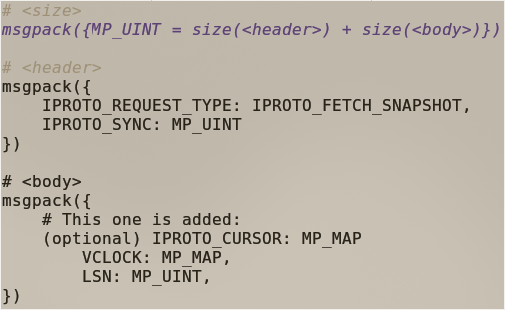
\includegraphics[scale=2.00]{inc/listing.png}
  \caption{Изменения в запросе IPROTO\_FETCH\_SNAPSOT}
  \label{fig:fig04}
\end{figure}

Добавляется новое поле в тело запроса: IPROTO\_CURSOR, представляющее собой таблицу с полями VCLOCK и LSN. Она указывает, откуда необходимо продолжить скачивание файла. Она может иметь следующие значения:

\begin{itemize}
    \item \textit{\{nil, nil\}} - используется скачивания read-view для обратной совместимости
    \item \textit{\{\{0\}, 0\}} - курсор неизвестен, мастер берет последний сделанный snapshot и посылает его.
    \item \textit{\{VCLOCK, LSN\}} - курсор известен реплике и она хочет продолжить скачивание. Находим snapshot, идентифицируемый vlock-ом и начинаем пересылку с определенного LSN.
\end{itemize}

Мастер при получении IPROTO\_CURSOR проверяет, что снапшот с запрашиваемым vclock-ом еще существует и что в нем есть запрашиваемый LSN. В противном случае реплике возвращается ошибка, она должна снова передать \textit{\{\{0\}, 0\}} и начать скачивание уже другого снапшота заново.
